\chapter{Discussion and Conclusion}
\label{discuss} % Always give a unique label

The results have shown that the developed system is linear and has high sensitivity, appropriate measuring range, high resolution, and low noise. In addition, the results from FFT analysis have shown that the developed PCB gives low noise output. The noise is outside frequency range of the original signal and can be easily filtered out using digital low pass filter.

At the same time, the sensory system have high absolute errors, high RMSE, low precision, and significant hysteresis. Figure \ref{fig:Syst_err} shows X-component of the force measured at the same time using X-Y device and using "actual force" data from the load cell. The error value changes simultaneously with rapid changes of the force applied. Taking into account, low noisiness of the system, plausible explanation of the fluctuations in the output signal is systematic errors. Important to note, that the errors could be related to high hysteresis of the sensors.

\section{Mechanical Design Issues}

The force-sensing devices were designed so they can easily fit the daVinci cannula and the sterile adapter. The tolerances are compensated by adjustment of the set screws, giving good modularity of the system.

One of the disadvantages is addition of the weight to the arm, that can alter robot performance. Taking into account, that the device will be placed close to the center of rotation of the robot arm, it will have minimal affect on the moment of inertia in comparison to sensors added to the grippers.

\begin{figure}[h]
	\begin{center}
	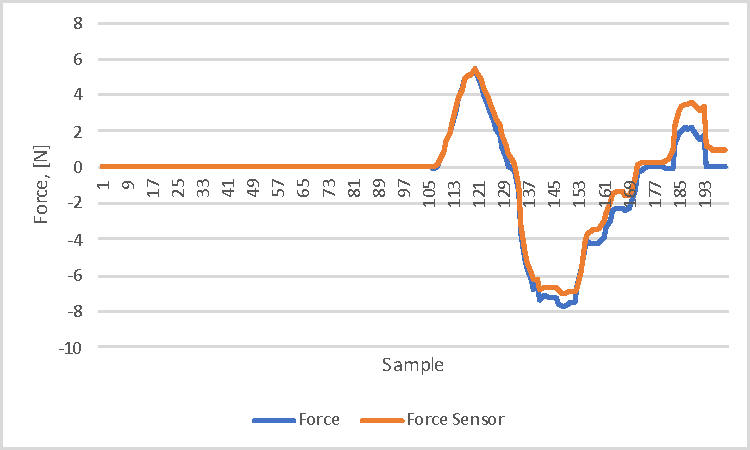
\includegraphics[width=100mm]{fig/results/syst_error.pdf}
	\end{center}
	\vspace{-4mm}
	\caption[Actual and Measured Forces in X-direction]
	{Actual and Measured Forces in X-direction}
	\label{fig:Syst_err}
	\vspace{-2mm}
\end{figure}

The calibration curve for Y-directional sensor has higher absolute error values, higher RMSE and lower linearity in comparison to X-directional sensor. The reason for that could be mechanical design issues caused by manufacturing problems (Figure \ref{fig:Syst_err_expl}). Different thicknesses of the walls, where sensors applied, cause different strain values for positive and negative directions of the force.

\begin{figure}[h]
	\begin{center}
	\includegraphics[width=100mm]{fig/results/device_bottom.png}
	\end{center}
	\vspace{-4mm}
	\caption[Y-direction Thickness of the Sensor]
	{Y-direction Thickness of the Sensor}
	\label{fig:Syst_err_expl}
	\vspace{-2mm}
\end{figure}

	Comparison of two Z-component of the force measurement methods have shown, that Z Device has lower signal-to-noise ratio, lower resolution, lower linearity, and higher hysteresis. Even though the joint effort method is slightly better than the created device, it does not comply to all sensor requirements, and it is hard to change the output results for this method. The major advantage of the created Z Device is ability to improve it. For example, hysteresis can be reduced by changing the force measurement plate material and its thickness.

The system has separate wheatstone bridges for each direction, giving the ability to measure each component of the force independently. However, Z Device and X-Y device cannot work together at the same time, because created X-Y device takes the Z-component of the force and slightly restricts rotation of the shaft. In order to solve that issue, we can change mechanical design of the X-Y device by increasing the size of the sleeve and adding slippery material between the shaft and the sleeve (Figure \ref{fig:NewXYDesign}). However, it will cause other issues with increased incision size to 1.9 cm. It is still in the appropriate range (1-2 cm) \cite{_laparoscopy}, however the patient recovery time would increase. Another option could be moving the X-Y device on the top of cannula or changing the cannula design and applying sensors on it.

\begin{figure}[h]
	\begin{center}
		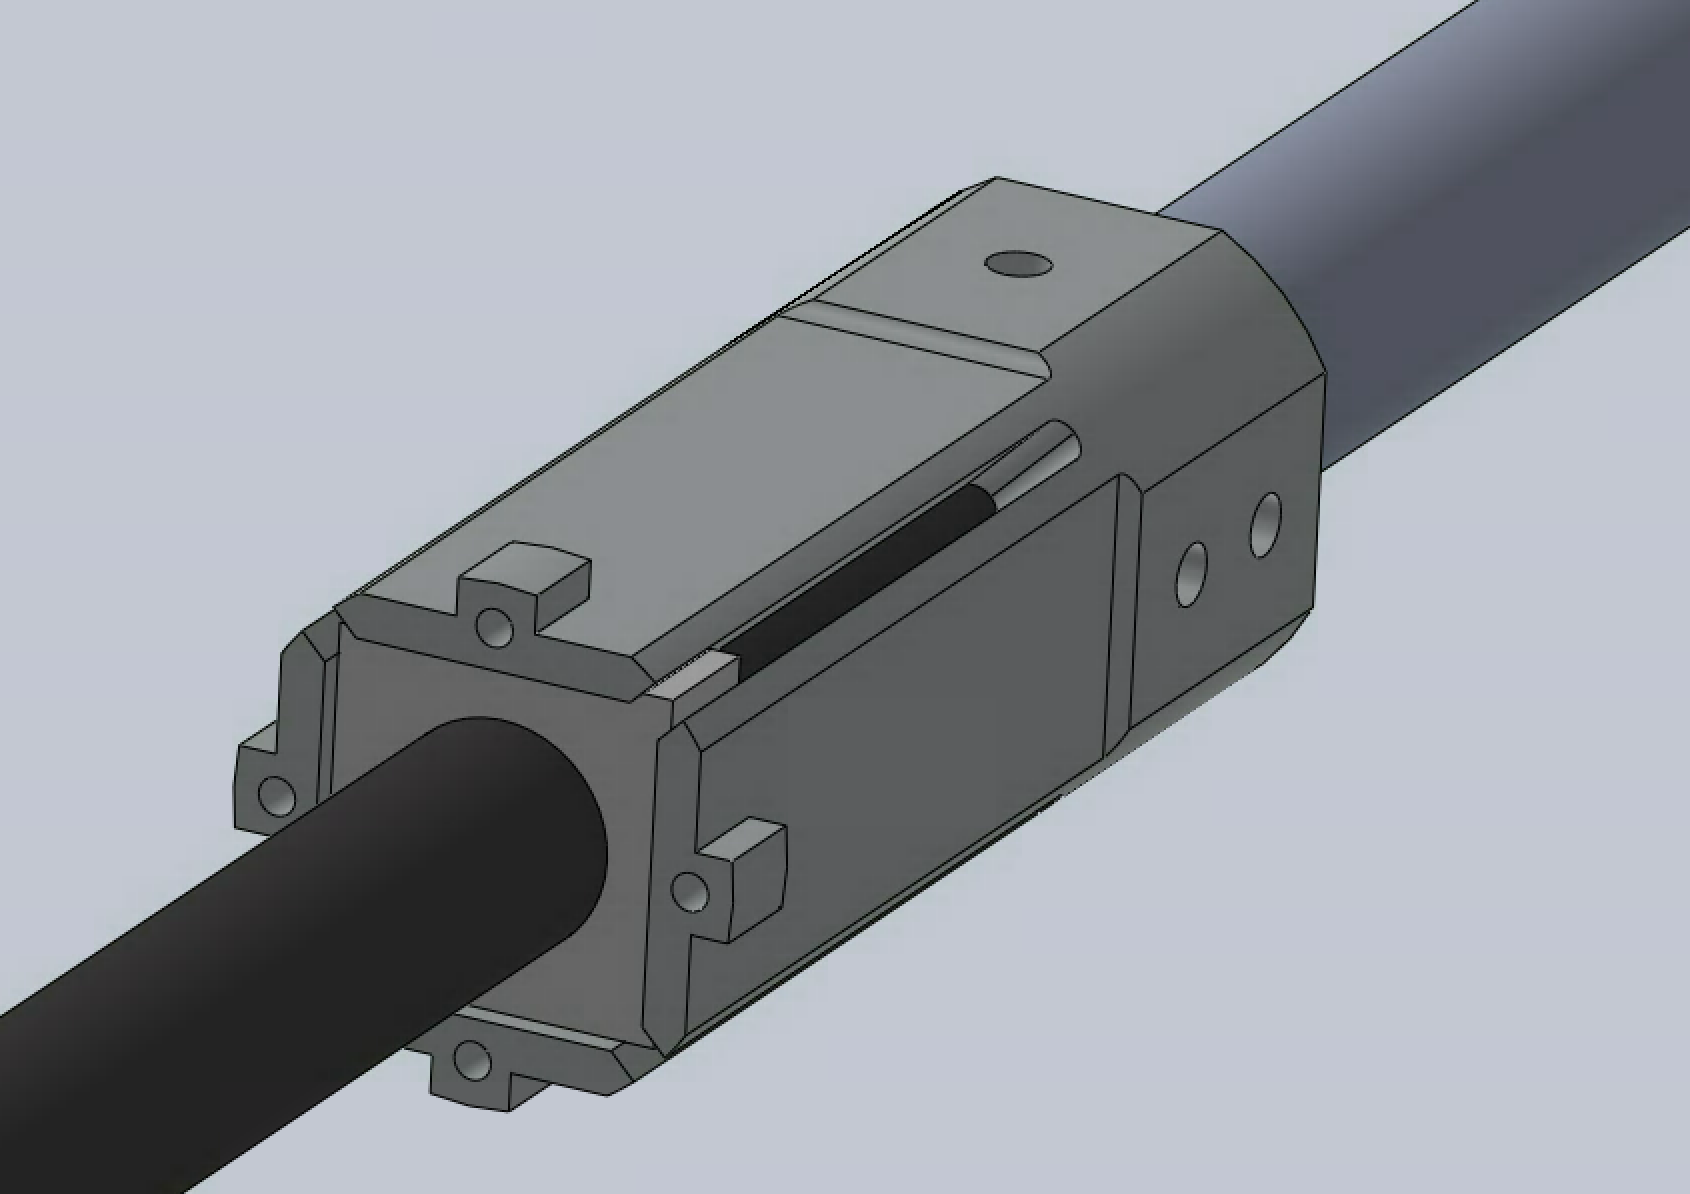
\includegraphics[width=120mm]{fig/methods/new_xy_dev.png}
	\end{center}
	\vspace{-4mm}
	\caption[New X-Y Device Design]
	{New X-Y Device Design}
	\label{fig:NewXYDesign}
	\vspace{-2mm}
\end{figure}
	
	Both devices should undergo sterilization. XY device goes inside the patient, meaning that it should be created using biocompatible materials. The current version of the device is not biocompatible. The biocompatibilty can be achieved using stainless steel as a device material and biocompatible epoxy to cover strain gauges, also teflon coated wires should be used for all electrical connections. Use of stainless steel will require change of the device dimensions, since the material has different elasticity.
	
\section{Electrical Design Issues}
	The real-time haptic feedback requires minimum data acquisition speed to be 1 kHz \cite{seungmoon_choi_effect_2004}. However, the current maximum speed is 588 Hz due to limitation of data transfer speed of serial communication (115.2 Kbps). In order to increase the speed, the communication channel can be changed to SPI (up to 10 Mbps) \cite{_uart_porotocol} or one of the wireless protocols, such as Bluetooth (up tp 1 Mbps) or wifi (up to 100 Mbps) \cite{_wireless_protocols}. Also, communication protocol between microcontroller and ADC can be changed from SPI to faster parallel communication. Additionally, the microcontroller can be changed to faster one, so it can support wireless communication. All these changes require change of the PCB design and microcontroller software. 
	
	Also, in the PCB the amount of Wheatstone bridges and ADCs should be increased from 2 to 4 to reduce the overall size of the system by removing second PCB and master-slave communication.
	
\section{Conclusion}

The created sensor gives 3-DOF force feedback. Showing that it is possible to add force-feedback in the daVInci robot without major changes of the existing system. However, not all of the requirements for the force measuring system were satisfied, meaning that the sensors need further improvements in both electrical and mechanical designs.